\documentclass[12pt, sumlimits, intlimits]{article}

\usepackage[utf8]{inputenc}
\usepackage[T1]{fontenc}
\usepackage[english]{babel}
\usepackage{hyperref}
\usepackage{lmodern, microtype}
\usepackage[top=3.5cm, bottom=2cm, right=2cm, left=3.5cm,
paper=a4paper]{geometry}
\usepackage[margin=2cm]{caption}
\usepackage{booktabs}
\usepackage{graphicx}
\usepackage{etoolbox}
\usepackage{color}
\usepackage{bm}
\usepackage{subfigure}
\usepackage{tikz}
\usetikzlibrary{shapes.geometric, arrows}
\usepackage[]{algorithm2e}

\usepackage{amsfonts, amsmath, amssymb}
\usepackage{mathtools}
\newcommand \yesnumber{\addtocounter{equation}{1}\tag \theequation}

\usepackage{listings}
\lstset{basicstyle=\footnotesize\ttfamily, tabsize=2}

\usepackage[backend=bibtex, style=authoryear]{biblatex}
%\addbibresource{refs.bib}
\addbibresource{../references.bib}

\setlength{\parindent}{0pt}
\setlength{\parskip}{2.5ex}
\pagenumbering{arabic}
\thispagestyle{empty}
\newcommand\todo[1]{{\color{red}!!!TODO: #1}}
\begin{document}


\includegraphics[width=8cm]{../figures/ecmi-logo.png}

ECMI Modeling Week 2018 \\*
University of Novi Sad, Faculty of Technical Sciences

\begin{center}
\vspace{2.0cm}
{\Large{\textbf{\MakeUppercase{The effect of clock drift on time delay data in a large network of seismic monitors}}}}

\vspace{\stretch{0.01}}

Christophe Picard University of Grenoble Alpes and Grenoble INP, France

\vspace{\stretch{0.01}}
\iffalse
\author{\thanks{} \and } \and  \and  \and 
\title{} 

\fi

\begin{tabular}{rl}
Jordi Anguera & Autonomous University of Barcelona, Spain \\
Leevi Annala & University of Jyväskylä, Finland \\
Stefan Dimitrijevic & University of Novi Sad, Serbia \\
Patricia Pauli & Technical University of Darmstadt, Germany \\
Liisa-Ida Sorsa & Tampere University of Technology, Finland \\ 
Dimitar Trendafilov & University of Sofia ''St. Kliment Ohridski'', Bulgaria

\end{tabular}

\begin{abstract}
	Seismic monitoring is used to study the behavior and composition of the underground floor. For earthquake prediction and underground works precise timing and positioning information is needed. Drilling companies use equipments that are linked in a network and are generally connected to a global positioning system for synchronization. However, instruments are not continuously  synchronized and their internal clocks may deviate in time. Hence, the periods to which the vibration of the underground floor are caught are inherently inaccurate due to inaccuracies in timing of the event. Consequently, the precise localisation of the events becomes impossible. In this study, we have time delay measurements and distance data of a seismic monitor network and we use it to investigate the time drift in each of the seismic monitor station clocks.
	
\end{abstract}
\vspace{\stretch{0.5}}


\today

\end{center}

\vspace{\stretch{0.15}}

\clearpage

\tableofcontents

\clearpage

\section{Introduction}

In operation of seismic networks high quality of data is required for accurate prediction of seismic events. Precise timing is crucial but continuous GPS synchronization of the stations' internal clocks is not possible due to high energy consumption. This is why we need to detect time drifts differently in times of disconnection from the GPS in order to continuously guarantee reliable data.

The purpose of this work is to analyze noise in a large network of seismic monitors and to extract clock drift from the delay.  This work suggests a way to determine clock drift based on the data only. For that, we use the information contained in the distance data to clear the delay data from clock drifts.

\section{Problem Statement}

\subsection{Definitions}
\begin{tabular}{c| p{11cm}}
	$\Delta_i$ & clock drift at station $i$\\
	$\delta_{ij}$ & Measured delay between station $i$ and station $j$ \\
	$\hat{\delta}_{ij}$ & Actual delay between station $i$ and station $j$ \\
	$\varepsilon_{ij}$ & Noise between two stations $i$ and $j$, including clock drift and ambient noise \\
	$r_{ij}$ & Distance between stations \\
	$w_{ij}$ & Adjacency matrix element, weight between two nodes
\end{tabular}

\subsection{Modelling time delay between seismic monitors}
The network of monitors can be modelled as a complete graph. The signal of each monitor is cross-correlated with other monitor signals, finally yielding time-delay data $\hat{\delta}_{ij}$ between each monitor. The time delay between the monitors comprise information on the real time the seismic wave travels between the monitors $\delta_{ij}$, the inaccuracies of the clock (time drift), and other noise affecting the measurement. The position of each seismic monitor in the network is available that can be used to compute the distances $r_{ij}$ between all stations.

\section{Data}

The data is collected from a network of 73 seismic monitor stations recording ground vibrations in the Southeast region of France. The average distance between two monitors in the network is $166$ km. The GPS coordinate position of each station in the network is known (Figure \ref{fig:monitornetwork}) and they each contain a clock which is synchronized to the GPS once a month. The seismic monitor sensor records compression and decompression as discrete values -1 and 1, respectively, every second. The sensor responds to any event in the area, be it an earthquake, tremor from road traffic, airplane or any other pressure wave which travels in the ground.

\begin{figure}[ht]
	\begin{center}   
		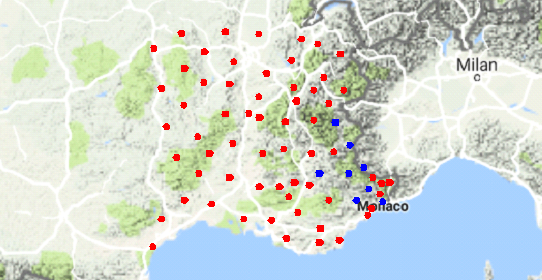
\includegraphics[width=0.6\textwidth]{../figures/TestStations_zoom.png}
	\end{center}
	\caption{The network of seismic monitors are located in the Southeast France, mostly in the regions of Provence-Alpes-C\^{o}te d'Azur and Rh\^{o}ne-Alpes. The eight stations chosen as the small test set is shown as green in the southeast part of the area.}\label{fig:monitornetwork}
\end{figure}

The stations work independent of each other and are occasionally shut down for some time frame for maintenance, repair or just random events. Just as occasionally they are brought back up to continue measuring.  Therefore, the number of active stations varies over time. The Figure \ref{fig:workingstations} shows the number of working stations, and the Figure \ref{fig:workingconnections} the number of working connections between the monitor stations over one year of measurements. 

\begin{figure*}[!ht] 
	\centering 
	\subfigure[The number of working seismic monitor stations.]{\label{fig:workingstations}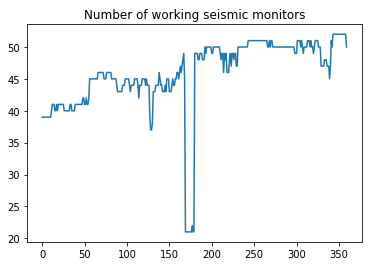
\includegraphics[width=0.47\linewidth]{../figures/working_monitors.png}}
	\subfigure[The number of working connections between the stations.]{\label{fig:workingconnections}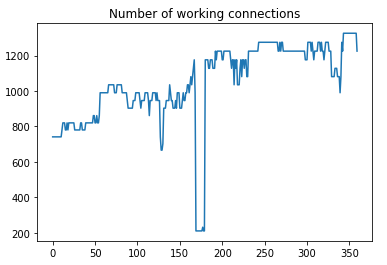
\includegraphics[width=0.49\linewidth]{../figures/working_connections.png}}
	\caption{Working stations and connections over one year time period. }
	\label{fig:workingmonitors}
\end{figure*}

\begin{figure*}[!ht] 
	\centering 
	\subfigure[Time Signal.]{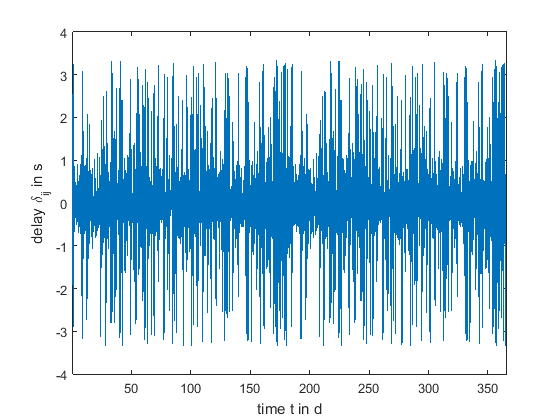
\includegraphics[width=0.49\linewidth]{../figures/delayevolutionovertimeforonestation2.png}}
	\subfigure[Histogram.]{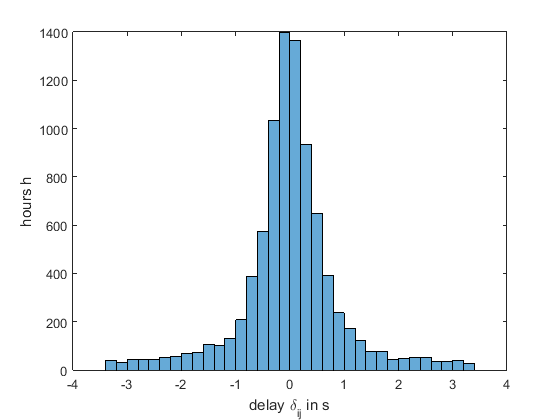
\includegraphics[width=0.49\linewidth]{../figures/delayevolutionovertimeforonestation.png}}
	\caption{The time-delay signal recorded between one station pair over a year. The time delay is computed in one-hour windows, yielding 24 time-delay values over a day.}
	\label{fig:examplesignal}
\end{figure*}

The compression and decompression data recorded by the stations is retrieved and run through initial data cleaning and filtering procedures. The data is then cross-correlated in one-hour time windows to yield time-delay data of signals between all monitors (Figure \ref{fig:examplesignal}). 

\begin{figure}[!ht]
	\begin{center}   
		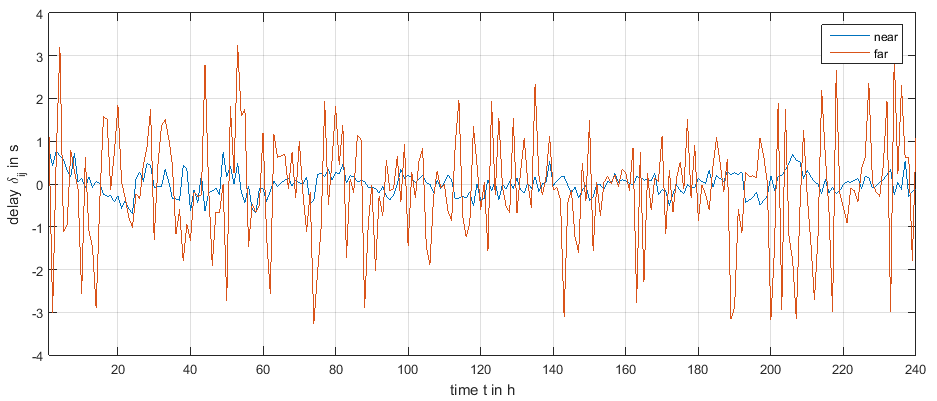
\includegraphics[width=\textwidth]{../figures/Comparisondelayoverrandomdayoffarestandclosestlinks.png}
	\end{center}
	\caption{Comparison of the delay of the furthest and closest station pairs over 10 days.}\label{fig:nearfar}
\end{figure}

The time delays between monitors are assumed to depend on the distance between the those same monitors. The further away the monitors are from each other, the longer the time a seismic wave travels from one station to  another. The time the wave travels corresponds to the actual delay and is the lion share of the measured delay between stations. Noise and clock drift are of a lower in order of magnitude. Figure \ref{fig:nearfar} shows the time signal of the station pairs that are closest and furthest apart over a time frame of 10 days supporting this assumption. One can see that the variance of the delays is much higher for the stations that are far apart. However the seismic events occur randamly.

\begin{figure}[ht]
	\begin{center}   
		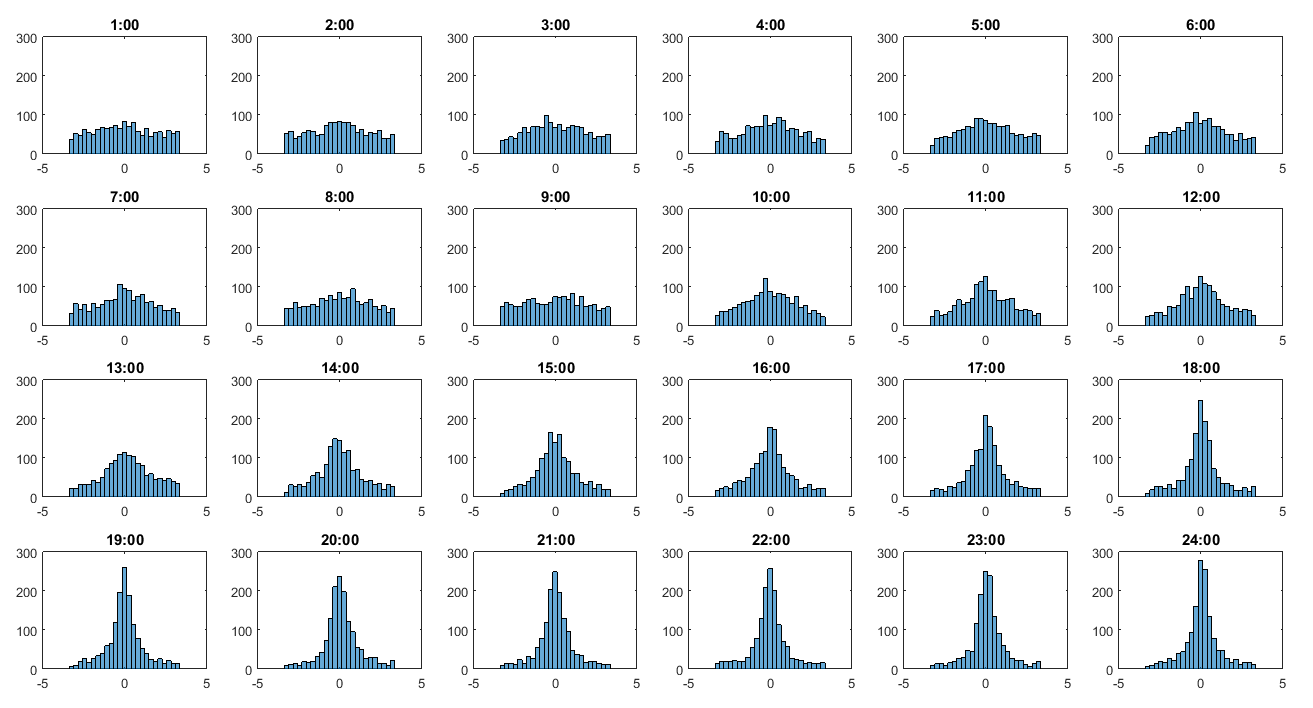
\includegraphics[width=\textwidth]{../figures/hourlydelaydistributionoverallstationsforoneday.png}
	\end{center}
	\caption{Histograms of time delays of all active stations recorded over 24 hours. The histogram shows how many connections have a particular delay at the instant.}\label{fig:histograms}
\end{figure}

The Figure \ref{fig:histograms} shows an example of time-delay evolution of all monitors over 24 hours. The distributions are symmetric with zero mean which implies that the delays at an instant cancel out over the whole area the 73 stations are mounted in. The interesting feature of the histograms is how the shape of the distribution changes slowly over time. However, the mean remains zero.


\subsection{The most influential stations}

The stations playing a key role in the global deviation of the total graph will be evaluated by the singular value decomposition of the global delays matrix $\bm{\hat{\delta}} \in\mathbb{R}^{n\times m}$, where $n$ is the number of edges and $m$ the number of time steps.

In order to find the index of the eigenvector with the most relative importance by the number of connections (regardless of the observed time delays) the time delay matrix $\bm{\hat{\delta}}$ was turned binary.

\begin{figure}[ht] 
	\centering 
	\subfigure[Singular values for the binary connection matrix.]{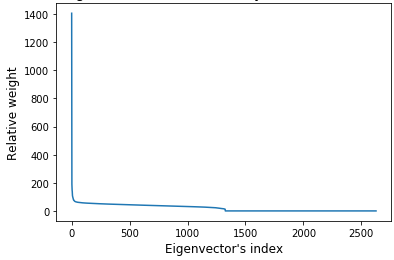
\includegraphics[width=0.49\linewidth]{../figures/singular_values.png} \label{fig:sing_va}}
	\subfigure[Influences of connections.]{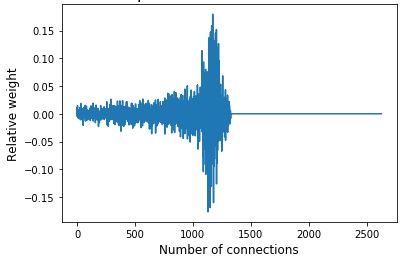
\includegraphics[width=0.49\linewidth]{../figures/connections_influence.png}\label{fig:influence}}
	\caption{Determining the influences of connections.}
	\label{fig:connectioninfluence}
\end{figure}

The Figure \ref{fig:sing_va} shows the relative weight of the connections for each of the eigenvalue's index, the first one being the largest one. With that, the next step was to find the connections with the largest relative weight and the limit at which the connections do not have any more influence in the overall time delay, which will be shown in Figure \ref{fig:influence} as a plot of the relative weight of each of the connections using the matrix $\bm{\hat{\delta}}$ with the measured time delays.

In order to select the group of connections with the largest weight a threshold of $|0.05|$ was taken, which resulted in 74 connections among 52 active stations. Finally, three stations with the largest numbers of connections (34, 21, and 13) were identified. The remaining stations had only two connections or less. 

These three stations were identified as the most influential stations, along with another group of five nearby these three stations stations, were taken as a small test set of stations to evaluate the methods developed in this work. 

\section{Methods}

Let $\bm{\hat{\delta}} \in \mathbb{R}^{n\times n}$ be the measured pairwise time delays of the system, $\bm{\delta}$ the actual pairwise time delays, and $\bm{\varepsilon}$ an error term including clock drift of the station's clock and other errors

\begin{equation}
\bm{\hat{\delta}}  = \bm{\delta} + \bm{\varepsilon}.
\label{eq:model}
\end{equation}

Each of the monitors are equipped with a clock which runs independent of others. It is synchronized via GPS system once a month and then runs independently. The inaccuracy in timing events at a station is caused by variations in the clocks' oscillators which oscillation may not be idea, they might respond to outside events and the oscillations are also affected by earthquakes. 

The position of each seismic monitor in the network is known. As the monitors are spread across a large area, it is assumed that local tremors are detected by stations that are close by, and therefore the correlations found in the pairwise cross-correlations and time delay data between them have higher likelihood to be linked. 

\subsection{The graph denoising model}\label{sec:denoising}
\subsubsection{Definitions}
The computational denoising model developed in this work involves weighted network estimation by the use of topological graph metrics, described in detail in \cite{Spyrou2017}. 

The monitor network constitutes a weighted graph $\mathcal{G}_{\delta} = (\mathcal{V}, \mathcal{E}, \bm{\hat{\delta}}_t)$ defined by a finite set of nodes $\mathcal{V}$ with $|\mathcal{V}| = n$, a set of edges $\mathcal{E} = \{ (v_i,v_j) \in \mathcal{V} \}$, with $\max |\mathcal{E}| = n^2-n$ and the weighted adjacency matrix $\bm{\hat{\delta}}$ with $\hat{\delta}_{ii} = 0$ for all $i$ based on the measured time delays between stations. The matrix $\bm{\hat{\delta}}$  is symmetric and describes the time delays between events in the graph, and is normalized, i.e. $\hat{\delta}_{ij}\in [0,1]$. The weighted adjacency matrix indicates the strength of connection between nodes.

The network also specifies another weighted graph $\mathcal{G}_r = (\mathcal{V}, \mathcal{E}, \bm{W})$, which sets of nodes and edges are the same as those of $\mathcal{G}_{\delta}$, but the adjacency weight matrix $\bm{W}$ is based on the physical distances between the station pairs. Also these weights are normalized between $[0,1]$.

\begin{figure*}[ht] 
	\centering
	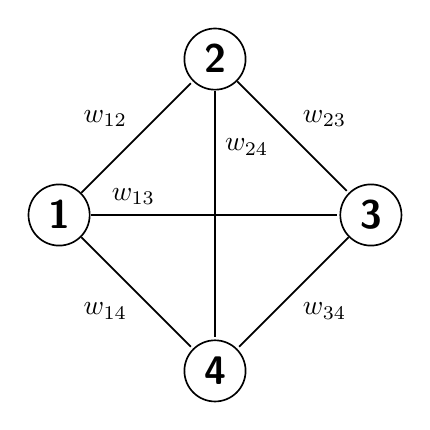
\begin{tikzpicture}[main node/.style={circle,draw,font=\sffamily\Large\bfseries},>=stealth',shorten >=1pt,auto,node distance=2.8cm,
	semithick]
	\tikzstyle{every state}=[draw=none]
	\node[main node] (1) {1};
	\node[main node] (2) [above right of=1] {2};
	\node[main node] (4) [below right of=1] {4};
	\node[main node] (3) [below right of=2] {3};
	\path (1) edge node {$w_{12}$} (2)
	edge node [above left, pos=0.3] {$w_{13}$} (3)
	edge node [below left] {$w_{14}$} (4)
	(2) edge node {$w_{23}$} (3)
	edge node [above right, pos=0.3] {$w_{24}$} (4)
	(3) edge node {$w_{34}$} (4);
	\end{tikzpicture}
	\qquad
	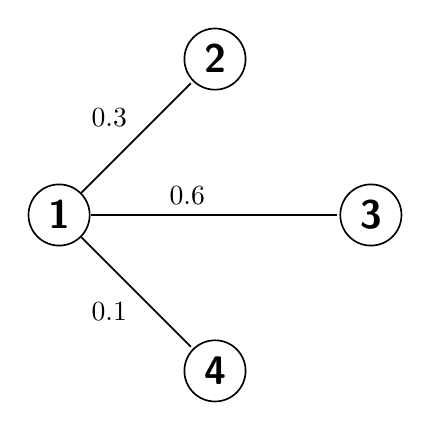
\begin{tikzpicture}[main node/.style={circle,draw,font=\sffamily\Large\bfseries},>=stealth',shorten >=1pt,auto,node distance=2.8cm,
	semithick]
	\tikzstyle{every state}=[draw=none]
	\node[main node] (1) {1};
	\node[main node] (2) [above right of=1] {2};
	\node[main node] (4) [below right of=1] {4};
	\node[main node] (3) [below right of=2] {3};
	
	\path (1) edge node {$0.3$} (2)
	edge node [above left] {$0.6$} (3)
	edge node [below left] {$0.1$} (4);
	\end{tikzpicture}
	\caption{Minimal example to help understand the computation of graph metrics.}
	\label{fig:graphmetrics}
\end{figure*}

\subsubsection{Graph metrics}
Graph metrics are scalar functions of the weight matrix $\bm{X}$ of a graph 
\begin{equation}
f_i(\bm{X})=K_i
\label{eq:metrics}
\end{equation}

They quantify a property of the network. In this work, the metrics involve time delays ($\delta_{ij}$) or the physical distances ($r_{ij}$) between stations. The connection strength of a node $i$ that is the row sum of the normalized weighted adjacency matrix: 
\begin{align}
f_i(\bm{\hat{\delta}})&=\sum_j\hat{\delta}_{ij} \quad \quad \quad \quad \quad \text{for }  \mathcal{G}_{\delta} = (\mathcal{V}, \mathcal{E}, \bm{\hat{\delta}}_t) \\
K_i &= f_i (\bm{W})= \sum_j{w_{ij}}  \quad \text{for }  \mathcal{G}_{r} = (\mathcal{V}, \mathcal{E}, \bf{W}).
\end{align}

The connection strength can be interpreted as the sum of all normalized delays of all of the connections to node i.

%
% The below is the earlier version of the distance metric
%\begin{figure}[htb]
%\centering
%\begin{tikzpicture}[xscale=0.45, yscale=0.3]
%\begin{scope}[shift={(0,2)}]
%\draw [-,very thick] (5,0) -- (8,4);
%\draw [-,very thick] (14,0) -- (8,4);
%\draw [-,very thick] (8,4) -- (13,5);
%\draw [-,very thick] (8,4) -- (3,8);
%\node[circle,fill,inner sep=2.5pt, label=above:$A$] at (8,4) {} ;
%\node [align=center] at (11,5) {\scriptsize 0.5};
%\node [align=center] at (5,7) {\scriptsize 0.1};
%\node [align=center] at (5.5,2) {\scriptsize 0.7};
%\node [align=center] at (12,2) {\scriptsize 0.2};
%\draw [-,very thick] (15,0) -- (20,4);
%\draw [-,very thick] (20,4) -- (25,4.5);
%\draw [-,very thick] (20,4) -- (16,8);
%\node[circle,fill,inner sep=2.5pt, label=above:$B$] at (20,4) {} ;
%\node [align=center] at (18,7) {\scriptsize 0.3};
%\node [align=center] at (16.5,2) {\scriptsize 0.1};
%\node [align=center] at (23,5) {\scriptsize 0.6};
%\end{scope}
%\end{tikzpicture}
%\caption{Distance metric.} \label{fig:1}
%\end{figure}

Figure \ref{fig:graphmetrics} shows a minimal example of how the metric is computed. The node $1$ has three connections yielding a connection strength $w_{12} + w_{13} + w_{14} = 0.1+0.3+0.6=1.0$. The other nodes and their connection strengths are computed similarly. 

Next, we look at the $K_i$. Since we have the distance measurements available and expect a correlation between the delays and distances, we want to use this information to denoise the delay measurements and define
\begin{equation}
K_i=f_i(\bf{W}).
\end{equation}
It is the connection strength as well. But here we plug in the distance matrix $\bf{W}$. The distances are constants and yield constant $K_i$.
The weight matrix $\bf{W}$ is a function of the distance between node $i$ and node $j$.
\begin{enumerate}
	\item First, we choose the function to be the reciprocal of the distances of the node to all other nodes, $w_{ij}= 1/r_{ij}$, normalized between $[0,1]$. Higher values correspond to nodes with short distances to all other nodes.
	\item Second, we try a metric with weights proportional to the distances ($w_{ij} \propto r_{ij}$), normailzed between $[0,1]$ accordingly. Here, high values correspond to long distances between two stations.
\end{enumerate}
Other possible metrics are average neighbor degrees (resilience), transitivity, or a clustering coefficient. The analysis based on these metrics is beyond the scope of this work.  


\subsubsection{Cost function}
We assume to have estimates of $M$ differentiable graph metrics, one for each node $i$, of the original matrix $\bm{\hat{\delta}}$, i.e. $f_i(\bm{\hat{\delta}}) = K_i$, where $i\in\{ 1,\dots, M \}$, then we can formulate a cost function that measures the deviation of the observed weight matrix's metrics $f_i(\bm{\hat{\delta}})$ to the estimates $K_i$ as: 
\begin{equation}
c(\bm{\hat{\delta}}) = \sum_i e_i^2(\bm{\hat{\delta}}) = \sum_i(f_i(\bm{\hat{\delta}})-K_i)^2
\end{equation}
The error is minimized with gradient descent updates on $\bm{\hat{\delta}}$: 
\begin{equation}
\bm{\hat{\delta}}^{(k+1)} = \bm{\hat{\delta}}^k-\mu\sum_i e_i(\bm{\hat{\delta}}^k)\frac{df_i(\bm{\hat{\delta}}^k)}{d\bm{\hat{\delta}}^k},
\label{eq:updates}
\end{equation}
where $k$ is the iteration index and $\mu$ the learning rate. %For the case of $m=1$, Equation \ref{eq:updates} describes the traditional single function gradient descent. 
We find the derivative for the gradient descent update step. For $i=2$ it is
\begin{equation}
\frac{df_2}{d\bm{\delta}}=\frac{\sum_j \hat{\delta}_{2j}}{d\bm{\hat{\delta}}}=
\begin{bmatrix}
0 & 1 & 0 & \dots  & 0 \\
1 & 0 & 1 & \dots  & 1 \\
0 & 1 & 0 & \dots  & 0 \\
\vdots & \vdots & \vdots & \ddots & \vdots \\
0 & 1 & 0 & \dots  & 0
\end{bmatrix}.
\end{equation}
It is a symmetric matrix with ones in the $i$th row and $i$th column. The diagonal entries remain zero.

\subsection{Clock drift estimate}

The denoising model in section \ref{sec:denoising} computes the denoised estimate $\bm{\delta}$ of the measurement data $\bm{\hat{\delta}}$. The algorithm is run over a series of time points and an estimate for the clock drift $\Delta_{ij}$ between each station pair is obtained. 

The noise, $\varepsilon_{ij}$, between each pair between two stations in the system is caused by clock drifts $\Delta_i$ and $\Delta_j$, and other ambient errors $E_{ij}$
\begin{equation}
\varepsilon_{ij} =  \Delta_i - \Delta_j  + E_{ij}.
\end{equation}
The unwanted ambient noise $E_{ij}$ is assumed to be white noise that can be cancelled out by interpolation of the total noise.


The clock errors of individual stations can be written in matrix form 

\begin{equation*}
\begin{bmatrix}
1 & -1 & 0 & 0 & \dots  & 0 \\
1 & 0 & -1 & 0 & \dots  & 0 \\
1 &  0  & 0 & -1 & \dots   & 0 \\
\vdots & \vdots & \vdots  & \vdots & \ddots & \vdots \\
1 &  0  & 0 & 0 & \dots & -1 \\
0 &  1  & -1 & 0 & \dots & 0 \\
0 & 1 & 0 & -1 & \dots & 0 \\
0 & 1 & 0 & 0 & \ddots & 0 \\
\hdotsfor{6} \\
0 & 0 & \dots & 0& 1 & -1
\end{bmatrix}
\begin{bmatrix}
\Delta_1 \\ \Delta_2 \\ \Delta_3 \\ \Delta_4 \\ \vdots \\ \Delta_k \\ \vdots \\ \Delta_{n-1} \\ \Delta_n
\end{bmatrix}
= 
\begin{bmatrix}
\Delta_1 - \Delta_2 \\ \Delta_1-\Delta_3 \\ \Delta_1-\Delta_4 \\ \vdots \\ \Delta_1 - \Delta_{n} \\ \Delta_2- \Delta_3 \\ \Delta_2 - \Delta_4 \\ \vdots  \\ \Delta_2-\Delta_k \\ \vdots \\ \Delta_{n-1} - \Delta_n
\end{bmatrix}
= 
\begin{bmatrix}
\Delta_{12} \\ \Delta_{13} \\ \Delta_{14} \\ \vdots \\ \Delta_{1n} \\ \Delta_{23} \\ \Delta_{24} \\ \vdots \\ \Delta_{2k} \\ \vdots \\ \Delta_{(n-1)n}
\end{bmatrix} , 
\end{equation*}

which can be written more compactly as

\begin{equation}\label{eq:Gs=m}
\mathbf{Gs} = \mathbf{m}
\end{equation}

where $s$ is the unknown model vector and $m$ the known data \cite{sens2008}. The matrix $\mathbf{G}$ has rank $n-1$, meaning that it is lacking full rank. 

This represents a classical overdetermined inversion problem which can be solved by ordinary least squares regression after Tikhonov reqularization. The ordinary least squares seeks to minimize the sum of squared residuals

\begin{equation}
\| \mathbf{Gs}-\mathbf{m} \|_2^2.
\label{eq:leastsquares}
\end{equation}

When Tikhonov regularisation is added to the Equation \ref{eq:leastsquares}, we obtain

\begin{equation}
\| \mathbf{Gs}-\mathbf{m} \|_2^2 + \| \bm{\Gamma}\mathbf{s} \|_2^2,
\label{eq:tikhonov}
\end{equation}

for some suitable Tikhonov matrix $\bm{\Gamma}$. We choose this matrix as a multiple of the identity matrix $\bm{\Gamma} = \alpha\mathbf{I}$, giving preference to smaller norms. 

The explicit solution is hence given by 
\begin{equation}
\hat{\mathbf{s}} = (\mathbf{G}^T\mathbf{G} + \bm{\Gamma}^T\bm{\Gamma})^{-1}\mathbf{G}^T\mathbf{m}.  
\end{equation}

\subsection{Algorithm}
The graph denoising algorithm by \cite{Spyrou2017} is described in algorithm \ref{alg:graphdenoising}. 

\begin{algorithm}[H]
	\KwData{Noisy data $W_e$, \\calculated estimates for graph metrics $K_m$,\\ learning rate $\mu$, \\maximum error $\epsilon$}
	\KwResult{Denoised data $\hat{W}$}
	initialization: $t = 0$, $W_0 = W_e$, $E = \sum_{m}(f_m(W_0) - K_m)^2$\\
	\While{$E > \epsilon$}{
		$W_{(t+1)} = W_t - \mu\sum_{m}(f_m(W_t) - K_m)\frac{df_m(W_t)}{dW_t}$\\
		\If{$w_{i,j} < 0$}{
			$w_{i,j} = 0$
		}
		\If{$w_{i,j} > 1$}{
			$w_{i,j} = 1$
		}
		$E = \sum_{m}(f_m(W_{t+1}) - K_m)^2$\\
		$t = t+1$
	}
	$\hat{W} = W_t$
	\caption{Graph denoising algorithm.}
	\label{alg:graphdenoising}
\end{algorithm}

The algorithm for obtaining the time delays for the measuring stations during time $t$ is described in algorithm \ref{alg:driftcalculation}.

\iffalse
\todo{ckeck inputs in algorithm 2. Shouldnt it be $\varepsilon$ only and the metrics belong in the other algorithm?}

\begin{algorithm}[H]
	\KwData{ measured time delays $\hat{\delta}$, \\calculated estimates for graph metrics $K_m$,\\ learning rate $\mu$, \\maximum error $\epsilon$, \\
	Tikhonov regularisation constant $\alpha$}
	\KwResult{Clock drifts $\Delta_i$}
	get $\delta$ by denoising the matrix $\hat{\delta}$ using algorithm \ref{alg:graph denoising} with four first input parameters\\
	get the errors between the stations by $\hat{\delta} - \delta$\\
	arrange the error matrix to match $m$ from equation \ref{eq:Gs=m}\\
	$\Delta = (G^TG + \alpha^2I^TI)^{-1}G^Tm,$ where $G$ and $m$ come from equation \ref{eq:Gs=m}, and $I$ is identity matrix of the size of $G^TG$. 
	\caption{Clock drift calculation.}
 	\label{alg:delaycalculation}
\end{algorithm}
\fi
\begin{algorithm}[H]
	\KwData{Results from algorithm \ref{alg:graphdenoising}, $\delta$, \\
		measured time delays, $\hat{\delta}$, and\\
		Tikhonov regularisation constant, $\alpha$.}
	\KwResult{Clock drifts $\Delta_i$}
	get the error matrix $\varepsilon$ between the stations by $\hat{\delta} - \delta$.\\
	arrange the error matrix $\varepsilon$ to match $m$ from equation  \ref{eq:Gs=m} and call it $m$.\\
	$\Delta = (G^TG + \alpha^2I^TI)^{-1}G^Tm,$ where $G$ comes from equation \ref{eq:Gs=m}, and $I$ is identity matrix of the size of $G^TG$. 
	\caption{Clock drift calculation.}
	\label{alg:driftcalculation}
\end{algorithm}

\section{Results}

The noisy time delay signal was analyzed by the graph denoising algorithm (Algorithm \ref{alg:graphdenoising}) and the clock drift was further processed by the Algorithm \ref{alg:driftcalculation}. The denoising of a signal between one station pair is depicted in the Figure \ref{fig:denoising}. For simplicity and readibility, the figure includes the signal for 10 days. The Figure \ref{fig:noisy10days} shows how the time delays between events between the pair of stations varies between roughly $[-3,3]$ seconds. The Figure \ref{fig:denoised10days} shows the denoised signal which, based on the assumptions introduced in the denoising algorithm, is the true time delay between observed events. The signal noise which includes also the clock drifts affecting this particular station pair is depicted in the Figure \ref{fig:noise10days}.  The figure \ref{fig:denoising} clearly shows how the signal and noise appear quite random and lacking trend by nature. 

\begin{figure}[ht] 
	\centering 
	\subfigure[Delay signal $\bm{\hat{\delta}}$ of one connection for 10 days.]{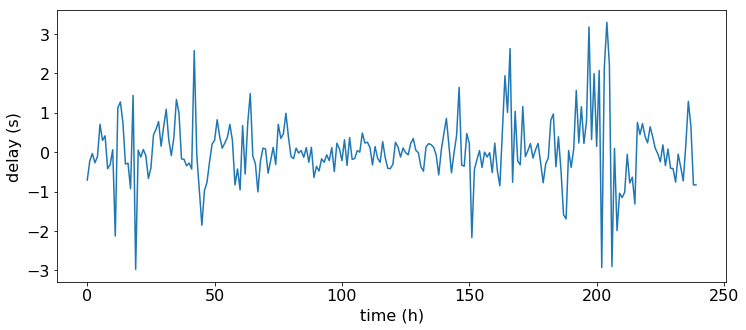
\includegraphics[width=0.49\textwidth]{../figures/noisy-time-delay-data-10-days.png} \label{fig:noisy10days}}
	\subfigure[Denoised signal $\bm{\delta}$ of the connection.]{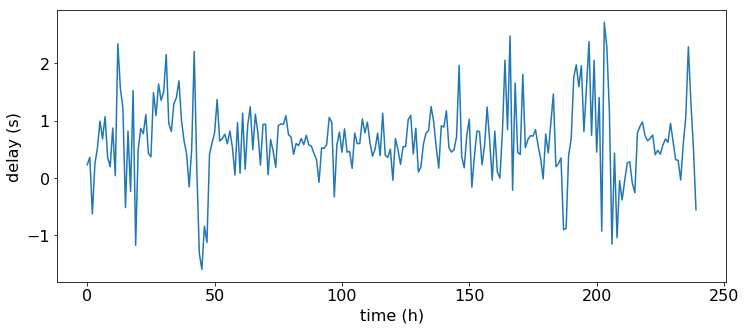
\includegraphics[width=0.49\textwidth]{../figures/denoised-time-delay-data-ten-days.png}\label{fig:denoised10days}}
	\subfigure[Signal noise $\bm{\varepsilon}$]{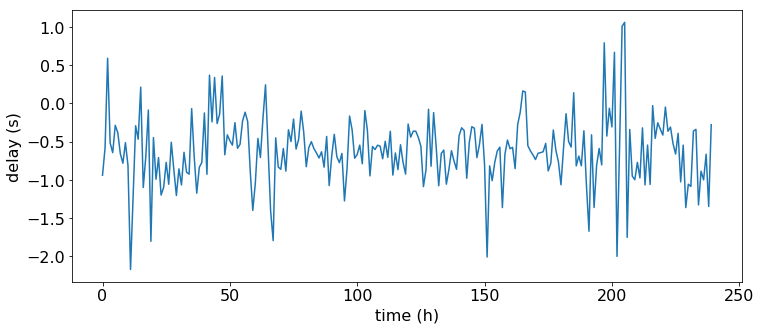
\includegraphics[width=\textwidth]{../figures/the-noise-ten-days.png}\label{fig:noise10days}}
	\caption{Denoising of the time delay signal at between two stations.}
	\label{fig:denoising}
\end{figure}

The clock drifts were obtained from the denoised signals such as the one depicted in the Figure \ref{fig:noise10days} and computed for each of the stations by using the Algorithm \ref{alg:driftcalculation}. The obtained clock drifts for each of the analyzed eight stations are shown in the Figure \ref{fig:clockdeviations}. It is evident in the figure that each of the station clocks tick at a different pace and that the pace varies. The scale of the axes are important. It shows that although an individual clock drift may account for up to 6 percent inaccuracy in timing at each time point, it may also tick at a roughly constant binary pace producing also binary deviation in the measurements, such as the clocks in the top and botton left in the Figure \ref{fig:clockdeviations}. 

\begin{figure}[ht]
\centering
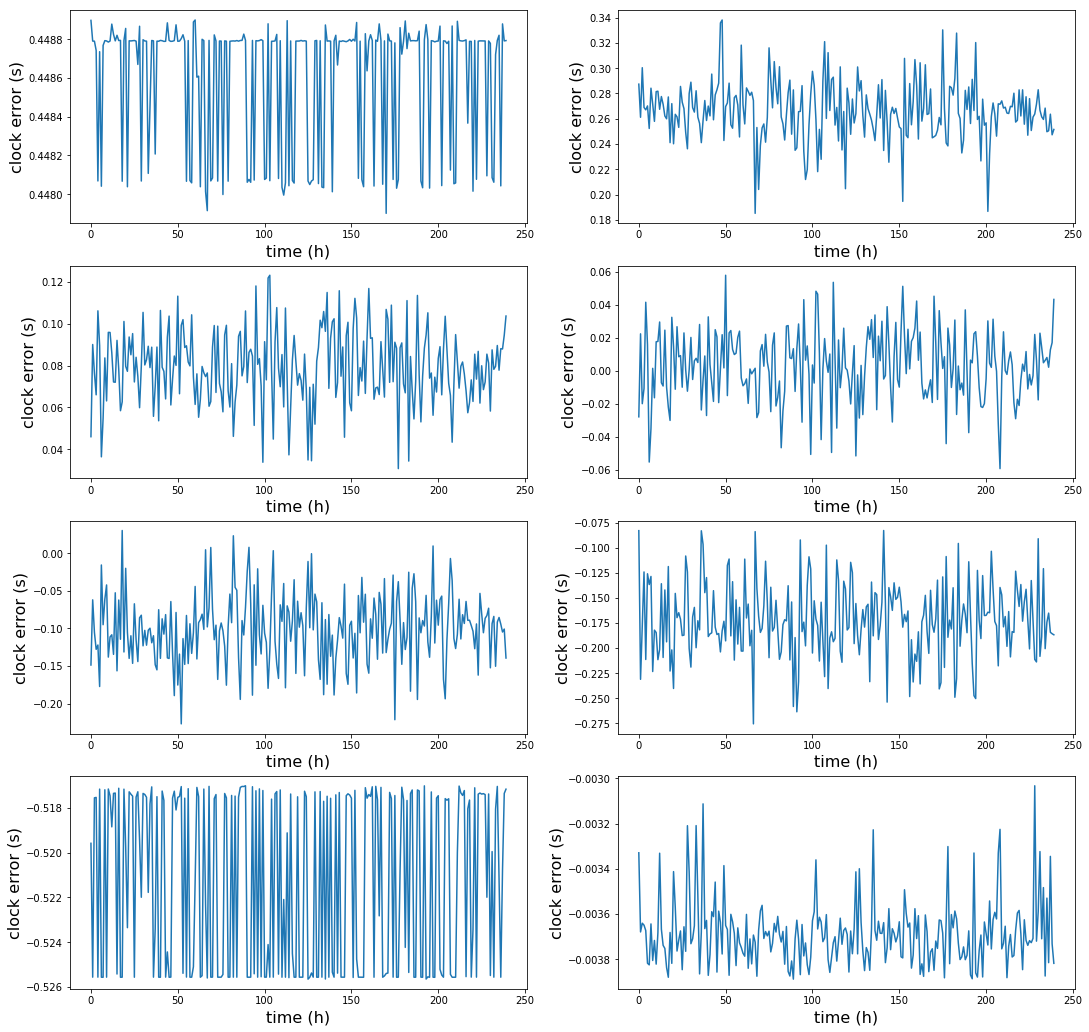
\includegraphics[height=0.9\textwidth]{../figures/results-for-eight-network.png}
\caption{Clock drifts of the eight stations obtained by the signal denoising model. The rough maximum scale of the individual clock drift is marked in the low right  corner of each figure.}
\label{fig:clockdeviations}
\end{figure}



\section{Conclusions and Outlook}
By analyzing the delay data we clearly showed that it changes over time showing patterns other than only white noise. This is due to clock drift. We used a method of weighted network estimation by the use of topological graph metrics exploiting the relation between delay and distances to denoise the data. The method is robust to temporarily disconnected stations that are only included as they are only included in the calculations when they are active. Hence, the algorithm can be run for on larger networks. The clock drifts are derived from the denoised time delay signals computed by the denoising algorithm developed in this work. 

The analysis provided in this report cannot produce conclusive evidence on the quality of the clock drift estimates due to missing validation data. This could be overcome by producing a synthetic dataset to first validate the methodology and then evaluate the obtained estimates. The methodology could be further augmented by developing other graph metrics in addition to the distance metric, or apply a combination of multiple metrics. As this work only included a subset of stations, the further work would also consist of including the complete network of stations in the analysis. 

%% Insert bibliography

\section{Group work dynamics}

Christophe gave us a more detailed presentation of the problem in the first group work session. After this, we asked questions and started a first discussion. From then on Christophe left the work and work distribution to us. We started by all absorbing the problem individually reading papers. The same afternoon we used the blackboard to discuss our ideas and find a feasible starting point for our work. Christophe had given us some assumptions and questions. 

The second day we decided to sit closer together in a circle and be closer to the blackboard that we kept using throughout the whole week to brainstorm ideas. 
We let everyone individually decide what they wanted to work on and sometimes asked around what everyone was currently working on to have a good overview and avoid that anything was left aside or the same thing was done twice. One subteam worked on the methods and developed the applied metrics, others analyzed the data and performed single value decomposition. This mode of working continued for the rest of the week. 

Some team members had more experience in group work than others and everyone had different backgrounds. This was an advantage in terms of the various view points and abilities we had as a group. However, communication was sometimes difficult as we didn't know what to expect from each other.

We started to write the report already during the week so we only needed to finalize details and write up results after the modelling week in Novi Sad. We stored our data, results, presentation and report in a GitHub project allowing for easy access and version control to all the team members. 

\section{Instructor's assessment}

Every instructor is asked to add a brief (1--2 paragraph) summary of how the
group has performed through the week, especially with respect to the problem's
initial goals and the actual achievements. Here is also the place to report
possible total or part-time absences of the students during the group work
hours --- these can be also reported by the fellow group mates.

\clearpage

\thispagestyle{empty}
\addcontentsline{toc}{section}{References}

% Possible references should be included in Harvard (author and year) style.

\printbibliography
%\bibliographystyle{abbrv}  
%\bibliography{references}   

\end{document}
